\documentclass[12pt]{exam}
\usepackage{amsmath, amssymb, amsfonts, amsthm}
\usepackage{graphicx}
\usepackage{hyperref}
\usepackage{tikz}
\usepackage{tikz-qtree}
\usepackage[margin=2.5cm]{geometry}
% \usepackage{fancyhdr} 


\usepackage{arabtex}

\usepackage{polyglossia}

\setmainlanguage{english}
\setotherlanguage{urdu}
\newfontfamily\urdufont[Scale=1.25]{jameel.ttf}




% \geometry{margin=0.5in, footskip=0.5in}

% \printanswers

\newtheorem{corrolary}{Corrolary}
\newcommand{\classX}[1]{\ensuremath{\text{\textsf{\textbf{#1}}}}} 
\newcommand{\classP}{\classX{P}}
\newcommand{\classNP}{\classX{NP}}
\newcommand{\NPC}{\classX{NP-complete}}
\newcommand{\coNP}{\classX{coNP}}
\newcommand{\EXP}{\classX{EXP}}
\newcommand{\coEXP}{\classX{coEXP}}
\newcommand{\PSPACE}{\classX{PSPACE}}
\newcommand{\NPH}{\classX{NP-hard}}
\newcommand{\T}{\text{\textbf{T}}}
\newcommand{\F}{\text{\textbf{F}}}
% \newcommand{\gcd}{\text{gcd}}}


\newtheorem{theorem}{Theorem}
\newtheorem{lemma}{Lemma}
\newtheorem{proposition}{Proposition}
\newtheorem{corollary}{Corollary}
\newtheorem{definition}{Definition}






\begin{document}


\pagestyle{plain}

\begin{minipage}[l]{0.1\textwidth}
		\noindent
		
\includegraphics[width=1.8\textwidth]{math club logo.png}
	\end{minipage}
\hfill
\begin{minipage}[c]{0.7\textwidth}
    \begin{flushleft}
    \Huge\texturdu{ مدرسہ ریاضیات }
    \vspace*{0.5cm}
    \\\Large Lecture 02 - The 3 Utilities Problem
    \\\large Habib Math Club
    \end{flushleft}

\end{minipage}
\newline
\bigskip
%%%%%%%%%%%% Please compile with XeLaTeX %%%%%%%%%%%%
%%%%%%%%%%%% Enter your text here %%%%%%%%%%%%

Imagine you are the Mayor of a town, and 3 people come to you one day arguing about something with much intensity. You ask them what the point of conflict is and one of them says:
\begin{center}
    "You see, Mayor, I moved in my house last week, and noticed that I was not getting any water. For a while I truged to the well and fullfilled my needs, but upon inquiry, I found out that these other houses were getting water all the same. Surprised, I ask for a connection to my house as well, but the other residents refused, saying it was not possible. I asked them their reasonsing and they said that it is forbidden in our town for any of the utility lines to ever meet each other, for a bad omen will spread on all the townspeople. I asked them to lend me a share in their connection, but once again they refused."
\end{center}


Can you, as the Mayor of the town, help the 3 residents resolve their conflict?

\begin{center}
    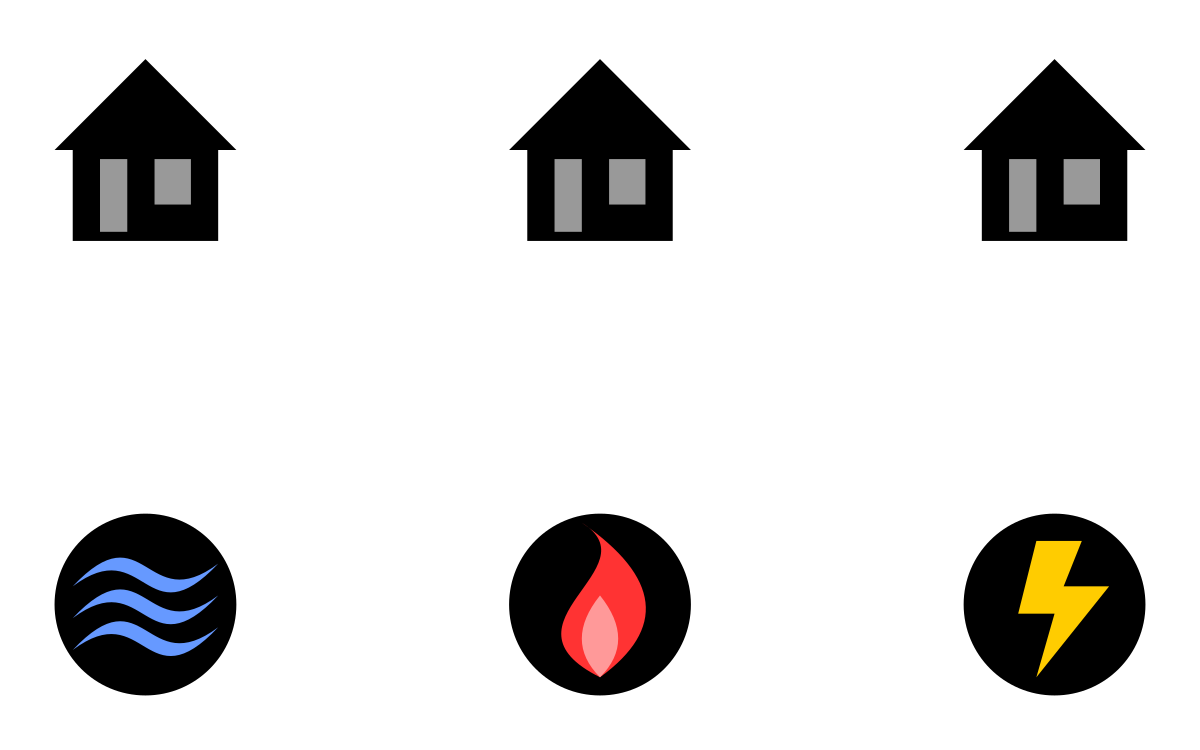
\includegraphics[width=0.7\textwidth]{3_utilities_problem_blank.svg.png}
\end{center}

\newpage

\section*{1. The History}

The utilities problem, also known as the water, gas, and electricity problem, is a classic puzzle, which goes back centuries. The current-known version of it asks whether it is possible to connect each of three utilities, Water (W), Gas (G), and Electricity (E), to each of three houses, A, B, and C, without any of the lines crossing one another.

Many variations of this puzzle have appeared over time, as mentioned by David Kullman in his paper [1]. In one version, the utilities are replaced by three wells, and the problem becomes the "Well-problem":
\begin{center}
    "Three persons live on adjacent lots, each provided with a well. Occasionally one or more of the wells run dry, so each person requires a path to each well. After a while the residents develop strong dislikes for each other and decide to construct their paths in such a way that they will avoid meeting each other on their way to and from the wells. Is such an arrangement possible?"
\end{center}

An even more dramatic version is the Corsican vendetta:

\begin{center}
    "There are three families such that any member of one family will attempt to kill any member of another family whenever their paths cross. However, the well, the market, and the church are, by tradition, neutral places which are free from violence. Therefore, the famiiies would like to take paths from their homes to the three safe places so that the paths of different famiiies will never cross."
\end{center}

The earliest known publication of the problem dates back to 1917. English puzzlist H. E. Dudeney stated it was “much older than electric lighting, or even gas,” but he provided no earlier references. Sam Loyd, Jr. claimed his father introduced (not invented) the puzzle in 1900. Historians believe the puzzle may date back even further!\\

Despite its simple nature, the utilities problem had been unsolved for decades. Most attempts at solving it involve tricks or loopholes, like allowing one line to pass through a house's basement. However, such tricks are not allowed in a plane, and it turns out, no solution exists (in a plane) without crossing lines. Dudeney eventually published a formal proof of this in 1926. [1]

\section*{2. What is a Planar Graph?}
A graph that can be drawn on a flat surface such that its edges do not cross each other (except at the vertices).\\

\begin{center}
    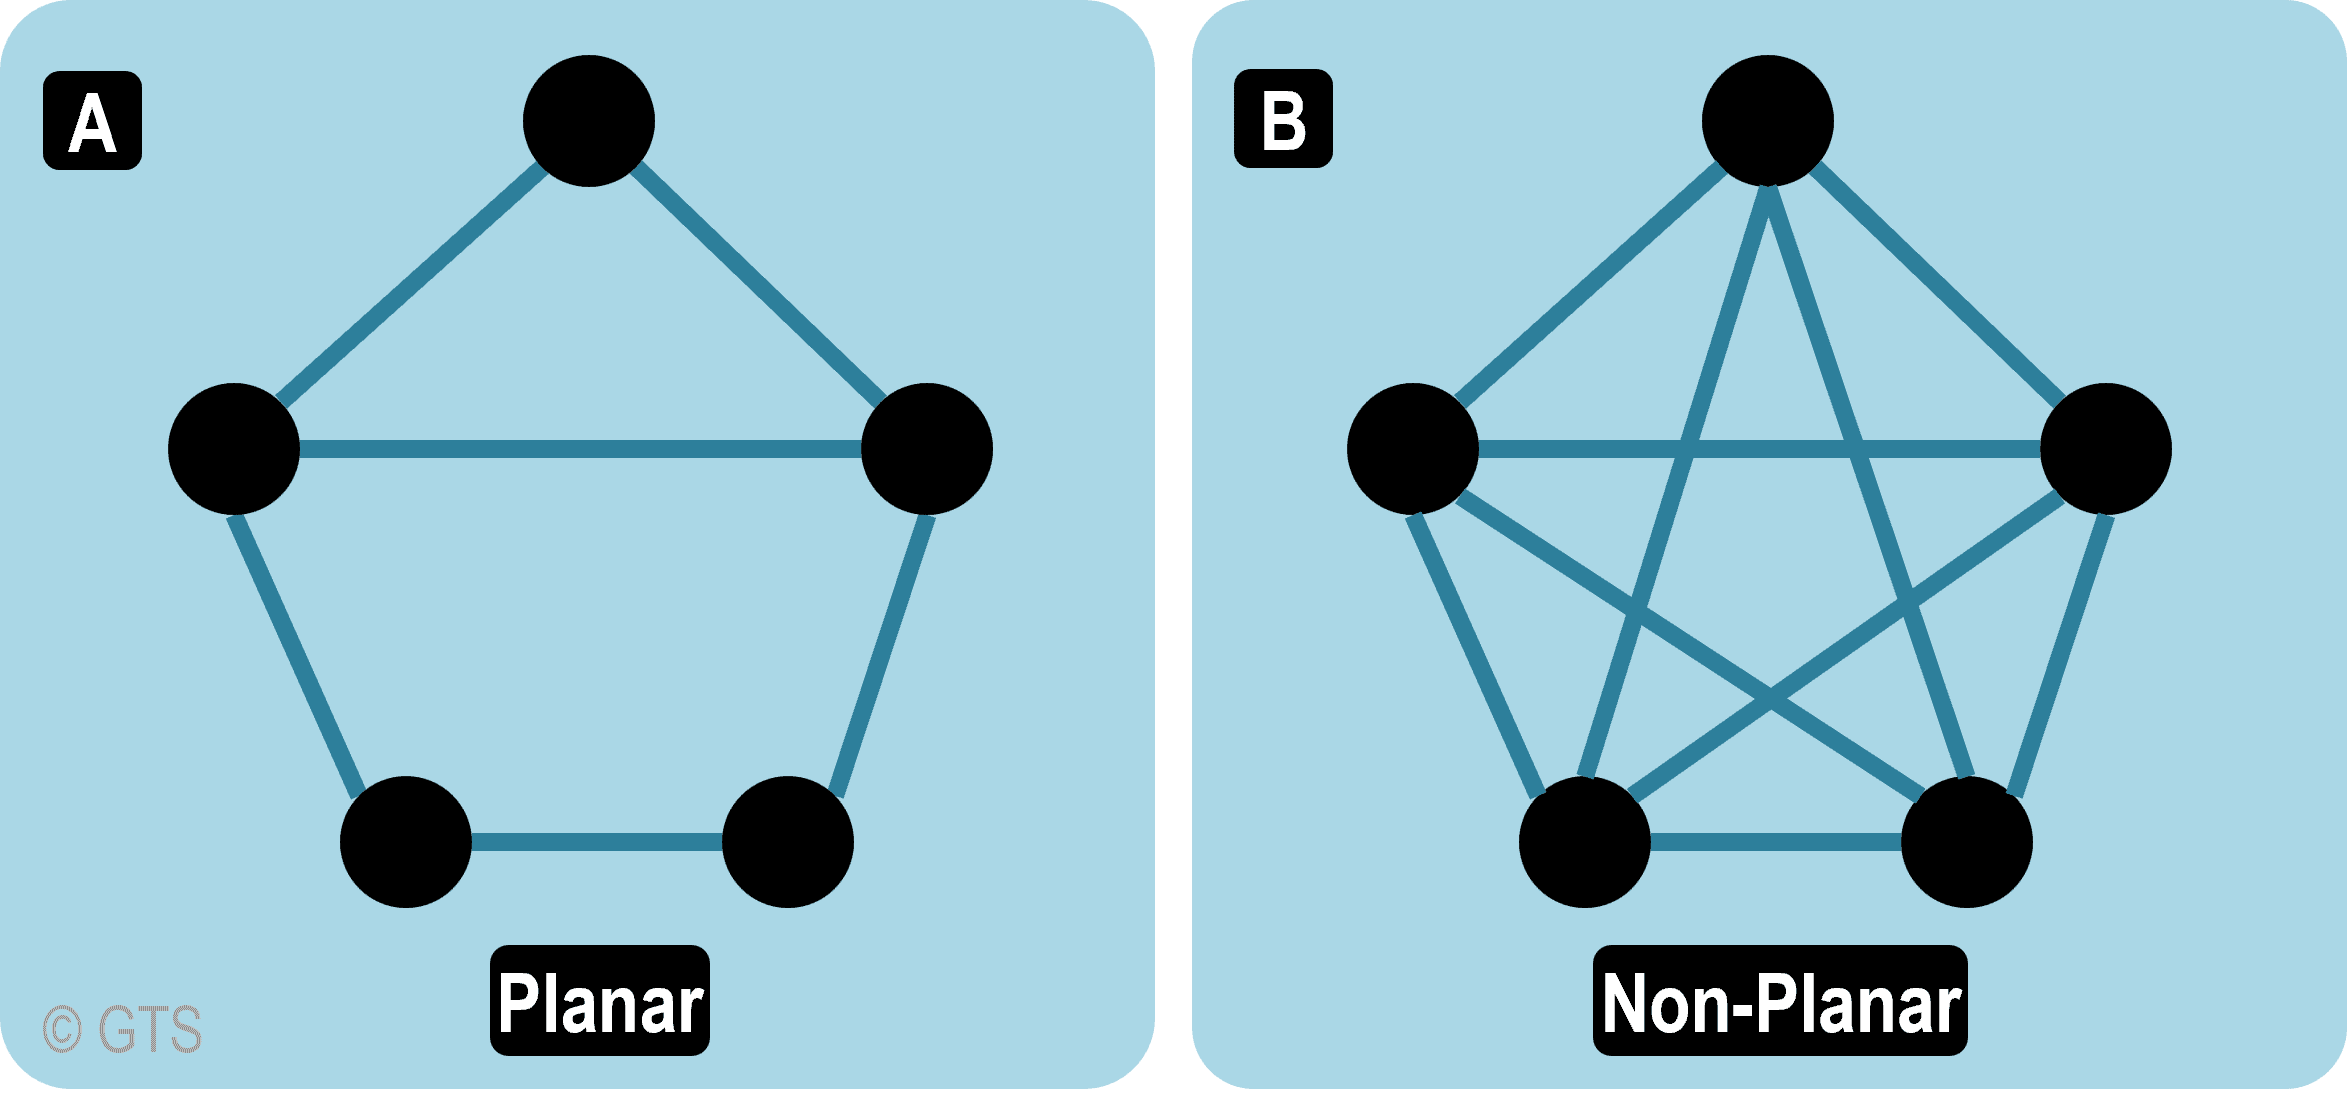
\includegraphics[width=0.7\textwidth]{planar_non_planar_graphs.png}
\end{center}

\textbf{Examples of planar graphs:}
\begin{itemize}
    \item A triangle
    \item A square
    \item A cube
\end{itemize}

\textbf{Examples of non-planar graphs:}
\begin{itemize}
    \item \textbf{K$_5$}: Complete graph with 5 vertices
    \item \textbf{K$_{3,3}$}: Complete bipartite graph with two sets of 3 vertices
\end{itemize}

\begin{center}
    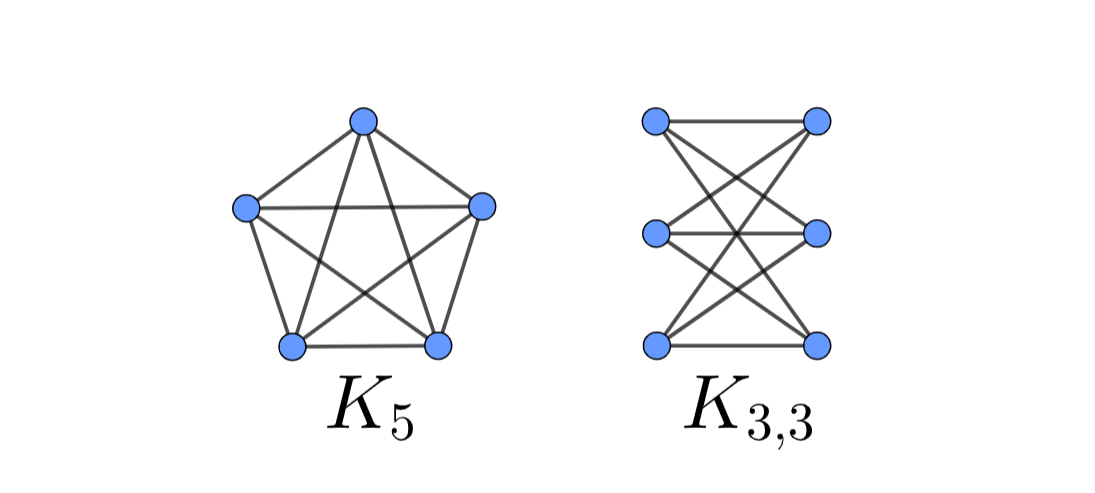
\includegraphics[width=0.7\textwidth]{k5.png}
\end{center}

\textbf{Complete Graph:}
A complete graph is a graph in which each vertex is connected to every other vertex.\\

\textbf{Bipartite Graph:}
A bipartite graph is a graph in which the vertex set, V, can be partitioned into two subsets, X and Y, such that each edge of the graph has one vertex in X and one vertex in Y.\\

In our 3 utilites problem, what we are basically asking is: \textbf{Is K-3,3 planar?}

\section*{3. What are Faces or Regions?}
In a planar drawing of a graph, the edges divide the plane into distinct areas called \textbf{faces} or \textbf{regions}. Each face is bounded by a cycle (when the ending and starting vertices of our path are same) of edges. The outermost region also counts as one face. The interesting thing about regions is that once enclosed, no new lines can enter or exit.\\

In the case of our utility problem, the minimum number of edges required to enclose a region has to be 4, because houses cannot be connected together and utilities cannot be connected to each other as well. It is important to note that each new edge drawn on our utility graph either is connected to a new vertex or creates a new region. Since we are ideally supposed to have 9 edges in our K-3,3 graph, an "ideal" solution would have 5 faces, not 4.

\section*{3. Euler's Formula (The Eulerian Characteristic)}
Euler's formula (which was initally derived for 3D shapes!) for connected planar graphs is:
\[
V - E + F = 2
\]
\begin{itemize}
    \item $V$ = number of vertices
    \item $E$ = number of edges
    \item $F$ = number of faces (including outer face)
\end{itemize}

\textbf{We can prove it by induction:}
\begin{enumerate}
    \item Base Case: A single vertes has $V=1$, $E=0$, $F=1 \implies 1 - 0 + 1 = 2$
    \item Inductive Step: Notice that adding an edge and vertex adds to $E$ and $V$ but it cancels each other out and keeps $V - E + F = 2$
\end{enumerate}

\section*{5. Handshaking Lemma for Faces}
In our planar graph, we know that:
\[
4F \leq 2E
\]
This comes from the idea that each face must have at least 4 edges (in the case of \textbf{K$_{3,3}$}) and that each edge touches 2 faces/regions. So one edge accounts for 2 faces.

\section*{6. Why K$_{3,3}$ is Not Planar}
In our utility graph, we know that:
\begin{itemize}
    \item $V = 6$, $E = 9$
    \item By Handshaking Lemma: $4F \leq 2E \implies 2F \leq E \implies F \leq \frac{E}{2}$
    \item Substitute this in Euler's Formula, we get: $V - E + \frac{E}{2} \geq 2$
    \item $2V - 2E + E \geq 2(2)$
    \item $2V - E \geq 4$
    \item $2(6) - E \geq 4$
    \item $12 - E \geq 4$
    \item $12 - 4 \geq E \implies 8 \geq E$
\end{itemize}
This is obviously a contradiction, since our graph has to have 9 edges, but this equation implies that only 8 edges or less are required. 
So $K_{3,3}$ is not planar.

\section*{7. Why K$_5$ is Not Planar}
Similarly, we can prove that K$_5$ is not planar:
\begin{itemize}
    \item $V = 5$, $E = 10$
    \item For this graph, the minimum number of edges for a cycle is 3, so our inequality becomes: $3F \leq 2E \implies F \leq \frac{2E}{3}$
    \item Substitute this in Euler's Formula, we get: $V - E + \frac{2E}{3} \geq 2$
    \item $3V - 3E + 2E \geq 2(3)$
    \item $3V - E \geq 6$
    \item $3(5) - E \geq 6$
    \item $15 - E \geq 6$
    \item $15 - 6 \geq E \implies 9 \geq E$
\end{itemize}
This is obviously a contradiction, since our graph has to have 10 edges, but this equation implies that only 9 edges or less are required. So $K_5$ is not planar.

\section*{8. Kuratowski's Theorem}
This leads us to a very interesting and important theorem, which states that:
\begin{center}
    "A graph is non-planar if and only if it contains a subgraph that is a subdivision of either \textbf{K$_5$} or \textbf{K$_{3,3}$}."
\end{center}
This theorem is used to classify any graph as planar or non planar.

\section*{9. Genus and the Torus}
The loophole with the mug was the fact that it was not a plane! It was a torus (donut-like shape), which allowed us to connect that final edge.
\textbf{Genus} is the number of "holes" in a surface. For example:
\begin{itemize}
    \item A plane or sphere has genus 0, as it doesnt contain any holes.
    \item A torus (like a donut) has genus 1. 
\end{itemize}


\begin{center}
    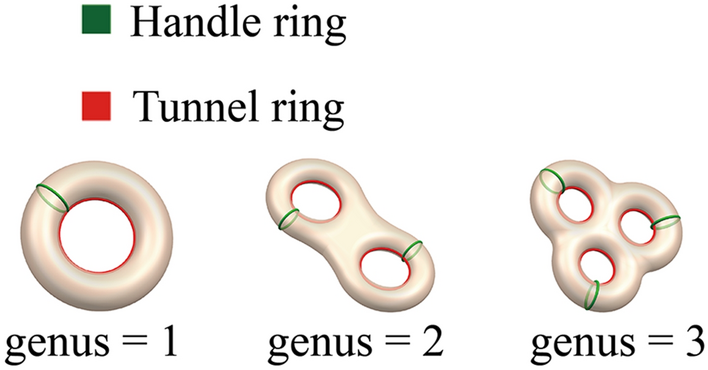
\includegraphics[width=0.7\textwidth]{genus.png}
\end{center}


Some non planar graphs can be drawn without crossings on surfaces with higher genus, which is why $K_{3,3}$ and $K_5$ can be drawn without crossings on a torus.

This explains why the 3 Utilities Problem is solvable when drawn on a mug: the handle acts like the "hole" in a torus, which allows that extra edge to finally connect!!\\

\vfill
\begin{center}
\small [1] Kullman, David E. “The Utilities Problem.” Mathematics Magazine, vol. 52, no. 5, Nov. 1979, p. 299, https://doi.org/10.2307/2689782. Accessed 18 Dec. 2020.
\end{center}





%%%%%%%%%%%% Replace with a Sher of your liking and uncomment this %%%%%%%%%%%%
% \vspace{2cm}
% \begin{center}
%     \texturdu{عشرتِ قطرہ ہے دریا میں فنا ہوجانا }
%     \\\texturdu{درد کا حد سے گزرنا ہے دوا ہو جانا }
%      \begin{flushleft}
%          \hspace*{4.5cm} (\texturdu{مرزا غالب })
%      \end{flushleft}
% \end{center}


\renewcommand\thefootnote{}


\renewcommand\thefootnote{\fnsymbol{footnote}}
\setcounter{footnote}{1}

% \nocite*{}

% \bibliographystyle{plain} 

% \bibliography{resource.bib}


\end{document}

% Template credit: Mujtaba Hassan





 


